\clearpage\setcounter{page}{1}\subsection[Приложения]{Приложения}
\hypertarget{Toc478978775}{}\subsubsection[Предисловие Издателя
(94)]{Предисловие Издателя
\textstyleEndnodeLink{(\ref{bkm:Ref474669698}}\textstyleEndnodeLink{)}}
\hypertarget{Toc478978776}{}\label{bkm:bm94}{\centering
(Леопольда фон Геннинга)
\par}

Автору «Науки логики» не было даровано закончить предпринятую им с большим
рвением новую обработку этого сочинения. Едва он успел написать последние
слова предисловия к I тому нового издания, как он был схвачен той болезнью,
печальный исход которой положил неожиданный конец его дальнейшей
деятельности на пользу столь мощно подвинутой им вперед науки. Хотя из
сравнения прежнего с новым изданием I тома этой «Логики» можно заключить, в
какой степени также и оба другие тома (перепечатываемые ныне с вышедшего в
свет в 1813 и 1816 гг. первого их издания) еще выиграли бы под рукой их
автора в строгости диалектического построения, в определенности выражения и
во внешней доступности, тем не менее нам служит немалым утешением
возможность сказать, что почившему великому учителю, предпринявшему эту
работу не без многолетней подготовки к ней и уже во вполне зрелом возрасте,
удалось уже в первоначальном ее выполнении создать сочинение, за которым
как уже и ныне, так еще более следующими поколениями будет признана слава
покоящегося на прочном фундаменте и во всех главных своих частях мастерски
выполненного органона мыслительного познания. Если, однако, не оказывается
недостатка и в таких друзьях истины, которые с полным признанием того, что
здесь сделано, считают необходимым несколько задержать свое суждение и
вообще не желают ничего знать о {\em готовой} системе
истины, так как, по их мнению, после такой системы для них и для дальнейших
поколений ничего не осталось бы делать (причем они имеют обыкновение
ссылаться на известное изречение
Лессинга)~\textstyleEndnodeLink{(}\label{bkm:bm95}\textstyleEndnodeLink{\ref{bkm:Ref474655210})},
то эти люди могут для своего успокоения в достаточной мере усмотреть из
предпринятой новой обработки этого сочинения, как обстоит дело с этой
внушающей опасение законченностью науки и каким образом ею нисколько не
исключаются новые достижения и успехи.—В каких границах наш покойный друг в
учениях о {\em сущности} и о
{\em понятии}, составляющих содержание второй и третьей
части настоящего сочинения, предпринял бы новую их обработку и какие новые
развитие и определения получили бы они, это в общих чертах можно усмотреть
из сравнения их с соответствующими отделами вышедшей в 1830 г. третьим
изданием «Энциклопедии философских наук». Из этого сравнения видно, что
автор, строго удерживая великие основные мысли своего сочинения, на
которые, по его собственному скромному заявлению, следует смотреть, как на
общий результат работ его предшественников в области философского познания,
и последовательно проводя метод, справедливо признанный им за единственно
правильный, сумел сохранить в себе потребные для живого прогресса науки
свежесть и подвижность духа. Пусть тем, которые призваны к дальнейшей
разработке нашей науки, служит постоянным образцом эта способность
самоотречения, это мужество разума и неутомимо стремившееся вперед рвение
дорогого учителя; и тогда не может возникнуть никакой основательной жалобы
на оцепенелость науки и на стеснение ее дальнейшего развития.

Задача издателя при перепечатке настоящего сочинения по самому существу дела
могла состоять лишь в тщательном исправлении найденных опечаток и описок, и
в этом отношении он в сомнительных местах позволял себе исключительно лишь
такие изменения, относительно которых он имел право быть вполне уверенным в
согласии автора, если бы была дарована возможность получить это согласие.

{\em Берлин}, 3 мая 1834 г.\textstylexxxviii{ }

\clearpage\setcounter{page}{1}\subsubsection[Примечания]{\textstylexxxviii{Примечания}}
\hypertarget{Toc478978777}{}
\bigskip


\bigskip

\begin{enumerate}
\item \label{bkm:Ref474654409}К стр. \pageref{bkm:bm01}. — Это примечание
прибавлено Гегелем в 1831~г., когда он подготовлял 2-е издание своей «Науки
логики».
\item \label{bkm:Ref474656094}К стр. \pageref{bkm:bm02}. — Это примечание
прибавлено Гегелем в 1831~г., когда он подготовлял 2-е издание своей «Науки
логики». Упоминаемое в нем 2-е издание «Феноменологии духа» Гегель не успел
подготовить к печати, так как внезапно умер 14 ноября 1831 г. Исправления
текста «Феноменологии» доведены были Гегелем лишь до 37-й страницы
«Предисловия». С этими исправлениями «Феноменология» была издана учениками
Гегеля в качестве II тома Собрания его сочинений (в 1832~г.). «Энциклопедия
философских наук» впервые вышла в 1817~г.: третье, расширенное издание ее
появилось в 1830~г., за год до смерти Гегеля.
\item \label{bkm:Ref474656170}К стр. \pageref{bkm:bm03}. — Гегель имеет в
виду философию природы Шеллинга, в частности сочинение Шеллинга «О мировой
душе» (1798~г.; 2-е изд. — 1806 г.; 3-е изд. — 1809~г.), в котором «закон
полярности» трактуется как «всеобщий мировой закон».
\item \label{bkm:Ref474656176}К стр. \pageref{bkm:bm04}. — А именно в
предисловии к «Феноменологии духа». В русском переводе под ред. Радлова
(Спб. 1913) это место гласит: «Известное вообще потому, что оно известно,
не является познанным» (стр.~14).
\item \label{bkm:Ref474656188}К стр. \pageref{bkm:bm05}. — Гегель цитирует
здесь в вольном переводе фразу из «Метафизики» Аристотеля (кн.~I, гл.~2,
982 b.). В русском переводе А. В. Кубицкого (М.—JI.~1934) это место
находится на 22-й стр.
\item \label{bkm:Ref474656193}К стр. \pageref{bkm:bm06}. — Там же, кн.~I,
гл.~1, 981~b. (в переводе Кубицкого стр.~20).
\item \label{bkm:Ref474656208}К стр. \pageref{bkm:bm07}. — Там же, кн.~I,
гл.~2, 982~b. (в переводе Кубицкого стр.~22). Гегель переставил предложения
в этой цитате.
\item \label{bkm:Ref474656355}К стр. \pageref{bkm:bm08}. — Ср. выше
замечание Гегеля об «экзотерическом учении кантовской философии» на стр.
\pageref{bkm:Ref474526580}.
\item \label{bkm:Ref474656376}К стр. \pageref{bkm:bm09}. — Гегель имеет в
виду философию И. Г. Фихте, который был еще жив, когда Гегель писал свою
«Науку логики» (1812).
\item \label{bkm:Ref474656390}К стр. \pageref{bkm:bm10}. — Имеется в виду
субъективный идеализм И.~Г.~Фихте.
\item \label{bkm:Ref474656395}К стр. \pageref{bkm:bm11}. — «Критика чистого
разума», предисловие ко 2-му изд., стр.~VIII (во 2-м изд. перевода
Лосского, Петроград 1915, стр.~9).
\item \label{bkm:Ref474656429}К стр. \pageref{bkm:bm12}. — Гегель имеет в
виду логические сочинения Христиана Вольфа (1679–1754) и его
последователей. К этому месту текста в 1-м издании «Науки логики» (Нюрнберг
1812) имелось следующее примечание Гегеля: «Одна только что появившаяся
новейшая обработка этой науки —~«Система логики» Фриса —~возвращается к
антропологическим основам. Крайняя поверхностность лежащего в основе этой
«Системы логики» представления или мнения самого по себе, а равно и его
разработки избавляет меня от труда в какой бы то ни было мере считаться с
этим лишенным всякого значения произведением». Упоминаемая в этом
примечании «Система логики» Я. Ф. Фриса (1773—1843) вышла 1-м изданием в
1811 г., 2-м изданием в 1819 г., 3-м —~в 1837 г.
\item \label{bkm:Ref474656465}К стр. \pageref{bkm:bm13}. — Имеются в виду И.
Г. Фихте и его единомышленники.
\item \label{bkm:Ref474656486}К стр. \pageref{bkm:bm14}. — Имеется в виду
метафизика Христиана Вольфа и его последователей.
\item \label{bkm:Ref474656514}К стр. \pageref{bkm:bm15}. — Имеются в виду
философские учения Фалеса (вода), Парменида (единое), Анаксагора (нус),
Платона (идея), Спинозы (субстанция), Лейбница (монада).
\item \label{bkm:Ref474656532}К стр. \pageref{bkm:bm16}. — Выражение
«тождество тождества и нетождества» очень характерно для Гегеля. Оно
встречается уже в ранней работе Гегеля «Различие между философскими
системами Фихте и Шеллинга» (1801 г.). См. Hegels Werke, hrsg. von Lasson,
Bd. I, S. 77 или Werke, hrsg. von Glöckner, Bd. I, S. 124. Это выражение
является как бы общей формулой гегелевской трактовки единства
противоположностей (согласно которой в {\em тождестве} противоположных
определений сохраняется, в снятом виде, также и {\em различие} между
ними), — в отличие от непосредственного, неподвижного тождества
противоположностей у Шеллинга, а также от «совпадения противоположностей в
боге» у Николая Кузанского, Гамана и других мистиков.
\item \label{bkm:Ref474656544}К стр. \pageref{bkm:bm17}. — Имеется в виду
философия И. Г. Фихте.
\item \label{bkm:Ref474656777}К стр. \pageref{bkm:bm18}. — В квадратных
скобках даются заголовки примечаний, приведенные у Гегеля в оглавлении
«Науки логики», но отсутствующие в самом тексте (см. замечание Ленина по
этому поводу в «Философских тетрадях», Москва 1933, стр. 122).
\item \label{bkm:Ref474656876}К стр. \pageref{bkm:bm19}, — В переводе
Лосского ({\em Кант}, Критика чистого разума, 2-е изд., пер. Н.
Лосского, Петроград 1915) это место, равно как и цитируемая ниже фраза,
даны на стр. 347–348. Курсив в цитируемой ниже фразе принадлежит Гегелю.
\item \label{bkm:Ref474656885}К стр. \pageref{bkm:bm20}. — Там же. Курсив
Гегеля.
\item \label{bkm:Ref474665318}К стр. \pageref{bkm:bm21}. — Имеется в виду
учение Фалеса о воде как первооснове всех вещей.
\item \label{bkm:Ref474665328}К стр. \pageref{bkm:bm22}. — Имеется в виду
пифагорейское учение о числах как сущности вещей.
\item \label{bkm:Ref474665342}К стр. \pageref{bkm:bm23}. — Приведенное в
тексте латинское двустишие взято из известной оды Горация «Justum et
tenacem propositi virum» (3-я ода 3-й книги), рисующей образ справедливого
и постоянного в своих намерениях человека, который ничего не боится и
которого ничто не может вывести из душевного равновесия.
\item \label{bkm:Ref474665370}К стр. \pageref{bkm:bm24}. — Среди многих
значений, которые имеет латинское слово «tollere», имеются такие
противоположные, как, с одной стороны, «возвышать», «возвеличивать», а, с
другой стороны, — «убирать», «устранять», «удалять». Соответственно с этим,
выражение «tollendum esse Octavium» заключает в себе двусмысленность: оно
может быть понято и как «следует возвысить Октавия» и как «следует убрать
Октавия».
\item \label{bkm:Ref474665385}К стр. \pageref{bkm:bm25}. — Гегель имеет в
виду латинское слово momentum (момент), которое он употребляет
приблизительно в том же значении, как и немецкое Aufgehobenes (снятое).
\item \label{bkm:Ref474665400}К стр. \pageref{bkm:bm26}. — Эта фраза в
издании 1833 г. (фототипически воспроизведенном Глокнером в 1928 г.) дана с
несколько необычными знаками препинания, что дало повод Лассону изменить
пунктуацию, прибавив тире перед словами «denn Sein hat...». Тем самым
глагол «ist» приобрел в главном предложении значение связки, тогда как
согласно пунктуации, даваемой в издании 1833 г., его следует понимать в
смысле самостоятельного глагола («имеется в форме» или, как переведено у Б.
Г. Столпнера, «имеет форму»). Если принять пунктуацию Лассона, то всю эту
фразу надо перевести так: «Это {\em целое} равным образом в форме,~т.~е.
{\em определенности} бытия (ибо бытие равным образом явило себя в
становлении имеющим характер всего лишь момента) есть нечто снятое,
отрицательно-определенное». Сопоставление этого места с серединой
\pageref{bkm:bm25a} стр. («Что целое, единство бытия и ничто, имеет
{\em одностороннюю определенность} бытия, — это является внешней
рефлексией») заставляет предпочесть интерпретацию Б. Г. Столпнера.
\item \label{bkm:Ref474665477}К стр. \pageref{bkm:bm27}. — Схоластический
термин «эминентно» (eminenter) обозначает наивысшую степень какого-нибудь
качества, свойства или какой-нибудь реальности.
\item \label{bkm:Ref474665489}К стр. \pageref{bkm:bm28}. — Выражение «omnis
determinatio est negatio» у Спинозы нигде не встречается. Встречается:
determinatio est negatio~—~в письме Яриху Иеллесу от 2 июня 1674 г. (см.
Спиноза, Переписка, М. 1932, стр. 173, письмо 50). Из всего контекста
письма, а также из сопоставлений с другими местами сочинений Спинозы
явствует, что слово «determinatio» означает в данном случае не
«определение», а «ограничение». Гегель вообще в значительной мере
произвольно толковал философию Спинозы. Основное искажение, которое он,
вслед за Шеллингом, допускал в оценке философии Спинозы, состоит в том, что
он не желал видеть в нем материалиста.
\item \label{bkm:Ref474665496}К стр. \pageref{bkm:bm29}. — Яков Беме
полагал, что немецкое слово Qual (мука) и латинское слово «qualitas»
(качество) происходят от одного и того же корня. В действительности корни у
них разные.
\item \label{bkm:Ref474665602}К стр. \pageref{bkm:bm30}. — Имеется в виду
кантианец Карл Шмид (1761–1812), философскую точку зрения которого Шиллер в
своем сатирическом стихотворении «Die Philosophen» выразил следующим
образом:\newline
Auf theoretischem Feld ist weiter nichts mehr zu finden,\newline
Aber der praktische Satz gilt doch: du kannst, denn du sollst!»\newline
(«В области теоретического разума нельзя ничего больше найти, но остается в
силе положение практического разума: ты можешь, потому что ты должен!»). У
самого Канта рассуждения на тему «ты можешь, потому что ты должен»,
встречаются как в «Критике чистого разума» (пер. Лосского, Пгр. 1915, стр.
442), так и в «Критике практического разума» (пер. Соколова, Спб. 1897,
стр. 37 и др.), а также и в других его произведениях.
\item \label{bkm:Ref474665621}К стр. \pageref{bkm:bm31}. — Лейбниц приводит
этот пример с магнитной стрелкой в «Теодицее» (часть I, § 50). Ср.
замечания Плеханова об этом примере в «К вопросу о развитии монистического
взгляда на историю» (Соч., т. VII, стр. 142–144).
\item \label{bkm:Ref474665661}К стр. \pageref{bkm:bm32}. — Немецкий текст
этой фразы после слова «следовательно» испорчен. Чтобы придать ему какой бы
то ни было смысл, приходится прибегать к тем или другим конъектурам. В
настоящем переводе положена в основу конъектура Б. Г. Столпнера, который
вместо слов «hiermit ein Perennirendes» предлагает читать «hiermit eines
perennirenden». Лассон предлагает другую конъектуру: он изменяет порядок
слов и вставляет неопределенный член «eines». Если принять конъектуру
Лассона, то это место надо будет перевести следующим образом: «...и,
следовательно, некоторого такого {\em наличного бытия}, которое
порождает себе в своем потустороннем опять-таки нечто продолжающееся во
веки веков и притом порождает его как от него отличное».
\item \label{bkm:Ref474665685}К стр. \pageref{bkm:bm33}. — Выражение «Was
für eines?» берется Гегелем как общий вид или общий тип таких выражений,
как «Was für Einer ist er?» (что он за человек?), «Was für ein Ding ist
das?» (что это за вещь?) и~т.~д. «Was für Eines ist das?» можно передать
по-русски словами: «Это что за штука?».
\item \label{bkm:Ref474665698}К стр. \pageref{bkm:bm34}. —См. прим.
\ref{bkm:Ref474665621} к стр. \pageref{bkm:bm31}.
\item \label{bkm:Ref474665714}К стр. \pageref{bkm:bm35}. — В немецком тексте
(как в издании Глокнера, так и в издании Лассона) вместо слова «nur» (лишь)
стоит «nun» (теперь). Повидимому, это опечатка.
\item \label{bkm:Ref474665735}К стр. \pageref{bkm:bm36}. — Немецкое слово
Quantitat (количество) образовано из латинского quantitas.
\item \label{bkm:Ref474665753}К стр. \pageref{bkm:bm37}. — Имеется в виду
юношеская философская работа Лейбница «О принципе индивидуализации»,
написанная им в 1663 г.
\item \label{bkm:Ref474665775}К стр. \pageref{bkm:bm38}. — {\em Кант},
Критика чистого разума, 2-е немецкое издание, стр.~449–450. Гегель
несколько перефразирует это место. Во 2-м издании перевода Лосского (Пгр.
1915) это место находится на стр.~263.
\item \label{bkm:Ref474665791}К стр. \pageref{bkm:bm39}. — В немецком тексте
вместо слов «nach denselben» (по ним,~т.~е. по этим моментам) стоят слова
«nach demselben» (по нему). Повидимому, это опечатка.
\item \label{bkm:Ref474665796}К стр. \pageref{bkm:bm40}. — В немецком тексте
вместо слова «quantitative» (количественное) стоит слово «qualitative»
(качественное). Повидимому, это опечатка.
\item \label{bkm:Ref474665804}К стр. \pageref{bkm:bm41}. — Имеются в виду
Шеллинг и его последователи в натурфилософии.
\item \label{bkm:Ref474665813}К стр. \pageref{bkm:bm42}. —Цитата взята с
предпоследней страницы «Критики практического разума» Канта.
Непосредственно перед этим находится известное место, начинающееся словами:
«две вещи наполняют душу всегда новым удивлением и благоговением... — это
звездное небо над нами и моральный закон внутри нас» (См. {\em Кант},
Критика практического разума, пер. Соколова, Спб. 1897, стр.~191).
\item \label{bkm:Ref474665836}К стр. \pageref{bkm:bm43}. — О «не-я» как о
«толчке» (Anstoss) Фихте говорит в начале третьей части своей книги «Основа
общего наукоучения» (1794 г.). В русском переводе «Избранных сочинений И.
Г. Фихте» (т.~I, М.~1916) о «толчке» говорится на стр. 226–227.
\item \label{bkm:Ref474665876}К стр. \pageref{bkm:bm44}. — Имеется в виду
шеллингова «система абсолютного тождества», как она развита главным образом
в сочинении Шеллинга «Изложение моей системы философии» (1801 г.).
\item \label{bkm:Ref474665904}К стр. \pageref{bkm:bm45}. — Намек на
сатирическое стихотворение Шиллера «Die Philosophen», 16-е двустишие
которого (под заголовком: «Вопрос о праве») гласит:\newline
«Jahrelang schon bedien ich meiner Nase zum Riechen;\newline
Hab ich denn wirklich an sie auch ein erweisliches Recht?»\newline
(«Уже в течение многих лет я пользуюсь своим носом для нюханья, но имею ли я
и в самом деле право на это —~право, которое можно было бы доказать и
обосновать?»).
\item \label{bkm:Ref474665953}К стр. \pageref{bkm:bm46}. —В немецком тексте
вместо «которого» (dessen) стоит «которой» (deren). Повидимому, это
опечатка.
\item \label{bkm:Ref474665962} К стр. \pageref{bkm:bm47}. — Фигуру двух
неконцентричных кругов (см. рис.), заимствованную у Декарта («Принципы
философии», часть~II, §~33), Спиноза изобразил, в виде виньетки, на
титульном листе своего геометрического изложения «Принципов философии
Декарта» (вышло в Амстердаме в 1663 г.), а не «Этики», как ошибочно
утверждает Гегель.
\begin{center}
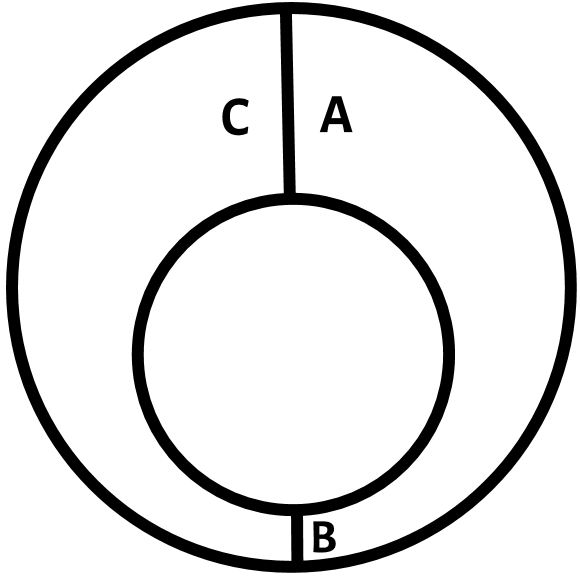
\includegraphics[width=1.25in,height=1.25in]{hegel-img002.png}
\end{center}
\item \label{bkm:Ref474665968}К стр. \pageref{bkm:bm48}. — Гегель дает здесь
в весьма вольном переводе и с перестановкой отдельных предложений
рассуждения Спинозы о бесконечном множестве неравных расстояний между двумя
неконцентричными окружностями (см. Спиноза, Переписка, М.~1932, стр.~78).
Конец приводимой Гегелем цитаты у Спинозы гласит: «...природа этой вещи не
может быть выражена никаким числом».
\item \label{bkm:Ref474666121}К стр. \pageref{bkm:bm49}. — В немецком тексте
вместо  стоит , а вместо  $(x+i)^n$ напечатано . Явная опечатка.
\item \label{bkm:Ref474666136}К стр. \pageref{bkm:bm50}. — Проверка с
помощью числа девять —~громоздкий искусственный прием, в настоящее время
вышедший из употребления, ввиду своей непрактичности.
\item \label{bkm:Ref474666147}К стр. \pageref{bkm:bm51}. — т.~е. «ведь эти
члены не будут иметь {\em никакого} значения» (или: «{\em никакого}
веса», «{\em никакой} силы»).
\item \label{bkm:Ref474666169}К стр. \pageref{bkm:bm52}. — См. стр.
\pageref{bkm:bm52a}–\pageref{bkm:bm52b}.
\item \label{bkm:Ref474666189}К стр. \pageref{bkm:bm53}. — Под
«Entwicklungspotenz» Гегель, как видно из этого места, а также из первого
абзаца следующего примечания («Еще другие формы, находящиеся в связи с
качественной определенностью величины», — стр. \pageref{bkm:bm53a}),
понимает то же самое, что в других местах он обозначает терминами:
«Entwicklungsglied» (член ряда, получающегося при разложении двучлена  по
формуле Ньютона), «Entwicklungsfunktion» (функция, получающаяся в
результате разложения в ряд,— «функция развертывания», как иногда
приходится переводить это выражение: см. напр. стр. \pageref{bkm:bm53b}),
«die Funktion der Potenzierung» (функция возвышения в степень),
«abgeleitete Funktion» (производная функция,— обычный в математике термин
для обозначения того, о чем здесь идет речь у Гегеля). Употребляя для
обозначения производной функции несколько странное выражение
«Entwicklungspotenz», Гегель, повидимому, хочет подчеркнуть существенное
значение того обстоятельства, что дело идет тут именно о {\em степенных}
функциях, о разложении по {\em степеням}, о том, что интересующая нас
переменная величина {\em имеет степень выше первой} (см. выше, стр.
\pageref{bkm:bm53c}). Поэтому как первоначальную, так и производную функцию
Гегель называет «{\em степенными} функциями» (Potenzenfunktionen).
\end{enumerate}
В связи с этим нельзя не привести отзыв Энгельса. В письме Марксу от 18
августа 1881 г. Энгельс, говоря о математических рукописях Маркса, замечает
по поводу математических примечаний Гегеля: «Старик Гегель... вполне
правильно угадал, говоря, что диференцирование в виде основного условия
требует, чтобы обе переменных имели различные степени и чтобы по меньшей
мере одна из них была во второй или ½-й степени. Теперь мы уже знаем
почему». ({\em Маркс} и {\em Энгельс}, Соч., т.~XXIV, стр.~531–532).

\begin{enumerate}
\item \label{bkm:Ref474666244}К стр. \pageref{bkm:bm54}. — См. прим.
\ref{bkm:Ref474666189}.
\item \label{bkm:Ref474666256}К стр. \pageref{bkm:bm55}. — В немецком тексте
вместо «verglichen» стоит «vergleichen». Повидимому, это опечатка.
\item \label{bkm:Ref474666305}К стр. \pageref{bkm:bm56}. —Здесь слово «нуль»
употребляется Гегелем в фигуральном смысле —~в том смысле, что сторона
обратного отношения перестает быть стороной отношения, если она становится
равной показателю. В математическом же смысле, если мы возьмем обратное
отношение, показателем которого является произведение членов отношения  и
приравняем один из членов отношения этому произведению (например, ), то
другой член отношения будет не нулем, а единицей (у = 1). В арифметическом
обратном отношении (о котором здесь у Гегеля еще нет речи и формулой
которого является $х+у=С$), действительно, если $х=C$,
то $у=0$.
\item \label{bkm:Ref474666541}К стр. \pageref{bkm:bm57}. — В немецком тексте
вместо «keine» (никакой) стоит «eine». Повидимому, это опечатка.
\item \label{bkm:Ref474666560}К стр. \pageref{bkm:bm58}. — В издании Лассона
эта часть фразы дается по 1-му изданию «Науки логики», где эта фраза
гласит: «И вот определенное количество, которое отныне уже не есть
безразличное или внешнее определение, а дано так, что оно вместе с тем
снято как такое определение...» и~т.~д.
\item \label{bkm:Ref474666566}К стр. \pageref{bkm:bm59}. — Гегель имеет в
виду философию Шеллинга.
\item \label{bkm:Ref474666577}К стр. \pageref{bkm:bm60}. — Английское слово
«фут» означает прежде всего «нога, ступня», а затем уже «фут» в смысле меры
длины, приблизительно соответствующей длине ступни человека
(30,5~{\em см}). То же самое имеет место и в немецком языке со словом
«Fuss».
\item \label{bkm:Ref474666643}К стр. \pageref{bkm:bm61}. — Слово «правило»
(die Regel) Гегель употребляет здесь в смысле «мерило», «масштаб», «норма»,
«образцовая или указная мера» (Massregel, Richtmass). В XVIII в. слово
«Regel» иногда употреблялось в смысле линейки с делениями. Гегель,
повидимому, и намекает на это старинное значение.
\item \label{bkm:Ref474666655}К стр. \pageref{bkm:bm62}. — Гегель
рассматривает здесь понятие физической {\em константы},~т.~е. того
эмпирического коэфициента, который в той или иной форме входит в уравнения
механики и физики. В качестве примера такой константы Гегель в следующей
фразе приводит величину $а$ в уравнении движения падения тел 
$s=at^2$. Гораздо чаще формулу движения падения тел
выражают уравнением $s=\frac 1 2 gt^2$, где константа
$g$ (постоянное для данного географического пункта ускорение силы
тяжести) равна приблизительно $9,8 \text{\em м}$ (в качестве единицы времени
берется при этом секунда). Следовательно, величина $а$ в уравнении
равна приблизительно $4,9 \text{\em м}$. Впрочем, надо сказать, что величина
$а$ или $g$, входящая в формулу движения падения тел, может
быть названа константою лишь в весьма относительном смысле. Дело в том, что
сама она изменяется с изменением расстояния от центра земного шара (а также
от расположения тяжелых масс на земной поверхности вблизи того места, где
производятся опыты с падением тел). Но так как эти изменения весьма
незначительны в тех случаях падения тел, которые рассматриваются в
элементарной механике (т.~е. в тех случаях, где расстояния, проходимые
падающим телом, незначительны по сравнению с длиной земного радиуса, причем
опыты производятся в одном и том же месте земной поверхности), то ими
вполне можно пренебречь.
\item \label{bkm:Ref474666676}К стр. \pageref{bkm:bm63}. —Здесь, как и в
предыдущем разделе «Мера как ряд отношений мер», Гегель имеет в виду учение
шведского химика Торберна Бергмана (1735–1784) о количественном выражении
сродства между основаниями и кислотами. Бергман предполагал, что одно и то
же количество какого-нибудь химического основания тем больше требует
кислоты для своего насыщения или нейтрализации, чем больше у них сродства
друг с другом. Он нашел, что для насыщения, например, 100 весовых частей
едкого кали требуется 78,5 весовых частей серной кислоты, или 64 весовых
частей азотной кислоты, или 51,5 весовых частей соляной кислоты и~т.~д.;
для насыщения же 100 весовых частей едкого натра нужно 177 весовых частей
верной кислоты, либо 135,5 весовых частей азотной кислоты, либо 125 весовых
частей соляной кислоты и~т.~д. В том и другом случае {\em порядок}
кислот остается {\em один и тот же}. Получается некоторой ряд пропорций
или мер насыщения (нейтрализации), который, по Гегелю, и характеризует
собой специфическую природу исследуемого вещества, выступающего в качестве
{\em противочлена} этого ряда. Учение Бергмана о химическом сродстве и
его количественном выражении было господствующей теорией в последней
четверти XVIII в. В начале XIX в. появилась новая теория химического
сродства, связанная с именем французского химика Клода Бертоллэ
(1748–1822), в значительной мере направленная против теории Бергмана.
Бертоллэ считал, что, наоборот, чем меньшее количество вещества $А$
требуется для нейтрализации вещества $В$, тем больше сродство между
ними. Кроме того, также и числовые значения мер насыщения, найденные
Бергманом, оказались при более тщательных экспериментах весьма неточными.
Сочинения Бергмана были изданы в немецком переводе в 1782–1799 гг. и были
широко известны в Германии. Между прочим, от Бергмана идет термин
«attractio electiva» (избирательное притяжение), который в немецком
переводе был передан термином «Wahlverwandtschaft» (избирательное
сродство), употребляемым здесь у Гегеля для обозначения одной из категорий
меры. Подробнее о теориях Бергмана и Бертоллэ см. у {\em Hermann Корр},
Geschichte der Chemie, Neudruck der Originalausgabe, Leipzig 1931, Bd. II,
S. 297–324, откуда и взяты вышеприведенные сведения. — Что касается
«избирательного сродства», как химической категории, то принцип этого
сродства был сформулирован еще задолго до Бергмана французским химиком
Этьеном Жоффруа (1672–1731), который в 1718 г. выставил следующее
положение: «Всякий раз, когда мы имеем соединение двух веществ, обладающих
склонностью соединяться друг с другом, если к этому соединению
примешивается третье вещество, имеющее более сильное сродство с одним из
первых двух, то это третье вещество соединяется с ним, отбивая его от
другого» (цитировано у Коппа, стр.~296 второго тома),~т.~е. указанное
третье вещество разлагает первоначально данное соединение, соединяясь с
одним из компонентов и вытесняя из соединения другой компонент.
\item \label{bkm:Ref474666698}К стр. \pageref{bkm:bm64}. — Имеется в виду
учение Бергмана (см. предыдущее примечание).
\item \label{bkm:Ref474666706}К стр. \pageref{bkm:bm65}. — «Учебник химии»
Берцелиуса вышел в трех томах в 1808–1828 гг.
\item \label{bkm:Ref474666715}К стр. \pageref{bkm:bm66}. — Гегель неправ:
причиной остановки маятника является не сила тяжести, а трение в том месте,
где маятник прикреплен или привязан, а также и сопротивление воздуха (или
какой-нибудь другой среды, в которой качается маятник).
\item \label{bkm:Ref474666719}К стр. \pageref{bkm:bm67}. — Немецкий текст
здесь испорчен. Перевод сделан на основе конъектуры Б. Г. Столпнера,
предлагающего вместо «eintretender qualitativer Bestimmtheit» читать
«eintretende qualitative Bestimmtheit». Лассон предлагает другую
конъектуру, вставляя перед указанными словами слова «ein Unterschied». В
этом случае надо было бы перевести эту фразу следующим образом: «Если,
таким образом, различие химического сродства, в противоположность
избирательному сродству, точно устанавливается в некотором ряде
количественных отношений, как различие появляющейся качественной
определенности...» и~т.~д.
\item \label{bkm:Ref474666725}К стр. \pageref{bkm:bm68}. — Имеются в виду
электрохимические теории английского химика Дэви (1778—1829) и шведского
химика Берцелиуса (1779–1848), явившиеся крупным шагом вперед в развитии
химии. Гегель недооценивал их значение, так же, как он недооценивал
прогрессивное значение химических теорий Бертоллэ.
\item \label{bkm:Ref474666740}К стр. \pageref{bkm:bm69}. — Выражение
«индиференция» (неразличенность, безразличие) было употреблено Шеллингом в
его вышедшей в 1801 г. работе «Изложение моей системы философии» для
обозначения «абсолютного тождества» субъекта и объекта. «Совершенная
неразличенность (totale Indifferenz) субъективного и объективного» —~таково
было основное понятие этой фазы философского развития Шеллинга. В
дальнейшем Гегель подробно рассматривает шеллинговскую концепцию
«индиференции как обратного отношения между ее факторами» и подвергает ее
имманентной критике, вскрывая ее «всестороннюю противоречивость». По учению
Шеллинга абсолютное представляет собою неподвижное тождество, полнейшую
неразличенность, совершенное безразличие двух факторов: субъективного и
объективного. Всякое же диференцирование состоит лишь в количественном
перевесе одного из этих двух факторов над другим, причем «вечным основанием
и опорою всех количественных различий субъективного и объективного служит
их совершенная индиференция, составляющая форму абсолютного тождества,
форму их бесконечного бытия» (см. {\em Куно Фишер}, Шеллинг, его жизнь,
сочинения и учение, пер. H. Лocского, Спб. 1905, стр. 590). О шеллинговой
системе «абсолютного тождества» Гегель упоминал также и выше, на
стр.~\pageref{bkm:bm69a}. Ср. прим.~\ref{bkm:Ref474665876} к этому месту.
\item \label{bkm:Ref474666761}К стр. \pageref{bkm:bm70}. — См. предыдущее
примечание.
\item \label{bkm:Ref474666774}К стр. \pageref{bkm:bm71}. — В первом издании
«Науки логики» (1812) здесь стояла еще следующая фраза, выпущенная Гегелем
в 1831 г., когда он готовил второе издание: «Этот вопрос я осветил в моей
более ранней диссертации, где я доказал несостоятельность этого различения
и построенных на нем объяснений». Имеется в виду «Философская диссертация
об орбитах планет» (1801) Возможно, что Гегель выпустил эту ссылку на свою
диссертацию потому, что в ней, между прочим, доказывалось, что между
Юпитером и Марсом не может быть никаких планет, между тем как еще в 1801 г.
была открыта малая планета Церера, расположенная как раз между Юпитером и
Марсом.
\item \label{bkm:Ref474666782}К стр. \pageref{bkm:bm72}. — Это не совсем
так. Как уже было упомянуто в примечании \ref{bkm:Ref474665489}{}-м, Гегель
в значительной мере произвольно толковал философию Спинозы, приписывая ей
акосмизм (отрицание мира) и идеализм. В этом отношении он шел по стопам
Шеллинга, использовавшего некоторые элементы спинозизма для построения
своей идеалистической философии «абсолютного тождества». В действительности
же между материалистом Спинозой и объективным идеалистом Шеллингом огромная
принципиальная разница, и эта-то разница как раз и смазывается в
гегелевской трактовке спинозизма.
\item \label{bkm:Ref474666794}К стр. \pageref{bkm:bm73}. —См. «Учение о
бытии», стр. \pageref{bkm:bm73a}—\pageref{bkm:bm73b}.
\item \label{bkm:Ref474666798}К стр. \pageref{bkm:bm74}. — В немецком тексте
вместо sie (т.~е. Negation) стоит es. Повидимому, это опечатка.
\item \label{bkm:Ref474666813}К стр. \pageref{bkm:bm75}. —См. примечание
\ref{bkm:Ref474665836}.
\item \label{bkm:Ref474666829}К стр. \pageref{bkm:bm76}. — См.
{\em Кант}, Критика способности суждения, пер. Н. Соколова, Спб. 1898,
стр. 16—17.
\item \label{bkm:Ref474666833}К стр. \pageref{bkm:bm77}. — Здесь кончается
выписка из «Критики способности суждения» (стр. XXVI немецкого издания 1799
г., стр.~16 русского перевода).
\item \label{bkm:Ref474666843}К стр. \pageref{bkm:bm78}. — Гегель имеет в
виду Шеллинга и его последователей. Шеллинг начиная с 1800 г., когда он
выпустил свою «Систему трансцендентального идеализма», выдвигает в качестве
«органа всякого трансцендентального мышления» «интеллектуальную интуицию»,
как непосредственное созерцание абсолютного, целиком противоположное
рассудочному познанию и совершенно оторванное от него. Против шеллинговой
«интеллектуальной интуиции» Гегель впервые выступил в начале 1807 г в
предисловии к «Феноменологии духа». В своих «Лекциях по истории философии»
Гегель дает более развернутую критику Шеллинга и его поклонников. Особенно
резко он отзывается об этих последних. «Вся эта тенденция, — говорит он об
антинаучном характере философских упражнений шеллингианцев, —
противопоставляет себя прежде всего {\em рефлективному мышлению}, или,
иначе сказать, такому движению рассуждения, которое держится фиксированных,
прочных, неподвижных понятий. Но вместо того чтобы оставаться в области
понятия и познать его как беспокойное «я», они впали в противоположную
крайность покоящегося созерцания, непосредственного бытия, неподвижного «в
себе» и полагают, что этот недостаток, эта неподвижность, исправляется
глядением и что это глядение они превращают в интеллектуальное, определяя
его в свою очередь посредством какого-нибудь фиксированного понятия»
({\em Гегель}, Лекции по истории философии, кн.~III. М.—Л. 1936,
стр.~511).
\end{enumerate}
Самое слово «рефлексия» Гегель употребляет в различных значениях, притом
так, что одно значение незаметно переходит у него в другое или даже
совмещается с другим. Латинское слово «reflexio» означает «загибание назад,
отклонение назад, отражение» (света, звуковой волны, брошенного во
что-нибудь предмета). В новых языках это слово наряду с этим значением
«отражения» приобрело еще значение «размышления, обдумывания, рассуждения,
соображения, рассудительности» (мысль как бы оборачивается на самоё себя,
отражается в себя самоё). У Гегеля рефлексия берется то в объективном, то в
субъективном смысле. При этом Гегель, как объективный и абсолютный
{\em идеалист}, понимает объективную рефлексию не в смысле взаимного
отражения сторон или моментов материального предмета друг другом или друг в
друге и не в смысле обратного их отражения в себя самих, а в смысле
взаимного отражения между определениями понятия как такового или в смысле
обратного отражения какого-нибудь понятийного определения внутрь себя
самого («рефлексия в себя»). Субъективную же рефлексию Гегель, как
идеалист, берет не в смысле гносеологического отражения объективно-реальной
материальной действительности в человеческом или животном сознании, а в
смысле рассудочного оперирования абстрактными категориями чистой мысли.
Рефлексия рассудка подвергается у Гегеля уничтожающей критике в том случае,
если она выступает с претензией на полное, завершенное, абсолютное
познание. Но вместе с тем Гегель решительно защищает эту рефлексию рассудка
как необходимый момент в диалектическом развитии познания (против Шеллинга
и шеллингианцев, против Якоби и против романтиков). Рефлексия в себя и
рефлексия в другое (притом не в другое вообще, а в «{\em свое} другое»)
составляют, по Гегелю, характерную черту категорий сущности (которая ведь
представляет собою «абсолютное опосредствование с собою»), точно так же как
переход от одного к другому был характерной чертой категорий бытия (где
господствует непосредственность), а развитие или развертывание
(Entwickelung) будет характерной чертой категорий понятия (где имеет место
единство непосредственного и опосредствованного).

В теснейшей связи с выражением «рефлексия» Гегель употребляет выражение
«Scheinen», имеющее у него опять-таки специфически-метафорическое значение.
«Das Scheinen» означает у Гегеля «свечение, мерцание, отблеск» (например,
Гегель говорит, что положительное «светится» в отрицательном, а
отрицательное —~в положительном; см. в тексте стр. \pageref{bkm:bm78a}).
Иногда Гегель приводит выражение «Scheinen» в прямою связь с термином
«Schein» (видимость, кажимость), и тогда «das Scheinen» приходится
переводить словами «свечение видимостью» (в себе самом или в своем другом),
или «излучение видимости» (в себя самого или в свое другое).

\begin{enumerate}
\item \label{bkm:Ref474666865}К стр. \pageref{bkm:bm79}. — В немецком тексте
(как в издании Глокнера, так и в издании Лассона) вместо слова
«положительным» стоит слово «отрицательным». Повидимому, это опечатка.
\item \label{bkm:Ref474666880}К стр. \pageref{bkm:bm80}. — В немецком тексте
наоборот: «+~а раз –~а». Повидимому, это опечатка.
\item \label{bkm:Ref474666891}К стр. \pageref{bkm:bm81}. — Об игре слов в
немецком выражении «zu Grunde gehen», как его употребляет Гегель, см.
замечания Энгельса в письмах Конраду Шмидту от 1 ноября 1891 г. и от 4
февраля 1892 г. ({\em Маркс} и {\em Энгельс}, Письма, под ред.
Адоратского, изд. 4-е, М.—Л. 1931, стр. 393–394).
\item \label{bkm:Ref474666904}К стр. \pageref{bkm:bm82}. — Слово «этиология»
(от греческого «aitia» —~причина, начало, основание) означает учение о
причинах, указание причин или оснований для тех или иных явлений.
\item \label{bkm:Ref474666911}К стр. \pageref{bkm:bm83}. — Лассон считает,
что придаточное предложение «что растение имеет свое основание в
производящей растения силе» попало сюда по ошибке и должно быть поставлено
двумя строчками выше, после слов «я скажу, что оно есть растение».
Стилистически такая перестановка улучшает конструкцию всей этой фразы, но
логический смысл заставляет предпочесть тот текст, какой дается в издании
Глокнера. С этого текста и сделан перевод этой фразы с добавлением слов
«того предложения» перед приведенным выше придаточным предложением.
\item \label{bkm:Ref474666923}К стр. \pageref{bkm:bm84}. — т.~е. по-своему,
по-разному.
\item \label{bkm:Ref474666940}К стр. \pageref{bkm:bm85}. — См. «Учение о
бытии», стр. \pageref{bkm:bm85a}–\pageref{bkm:bm85b}.
\item \label{bkm:Ref474667017}К стр. \pageref{bkm:bm86}. — В русском
переводе под ред. Радлова ({\em Гегель}, Феноменология духа, Спб. 1913)
это место находится на стр. 72—74 (в главе «Сила и рассудок, явление и
сверхчувственный мир»).
\item \label{bkm:Ref474667030}К стр. \pageref{bkm:bm87}. — В немецком
тексте: «das Relative eines Ändern». Повидимому, это опечатка вместо: «das
Relative seines Ändern».
\item \label{bkm:Ref474667041}К стр. \pageref{bkm:bm88}. — См. часть первая,
стр. \pageref{bkm:bm88a}–\pageref{bkm:bm88b}.
\item \label{bkm:Ref474667057}К стр. \pageref{bkm:bm89}. — В немецком
тексте: «in derselben». Повидимому, это опечатка вместо: «in demselben».
\item \label{bkm:Ref474667072}К стр. \pageref{bkm:bm90}. — Ср. замечание
Энгельса о том, что «сила имеет точно такую же величину, как и ее
проявление во-вне, ибо в них обоих совершается {\em одно и то же
движение}» ({\em Engels}, Herrn E. Dührings Umwälzung der Wissenschaft.
Moskau —~Leningrad 1935, S.~64).
\item \label{bkm:Ref474669620}К стр. \pageref{bkm:bm91}. — См. примечания
\ref{bkm:Ref474665489} и \ref{bkm:Ref474666782}.
\item \label{bkm:Ref474669634}К стр. \pageref{bkm:bm92}. — Это не точно. 4-я
дефиниция первой части «Этики» гласит: «Под атрибутом я разумею то, что
интеллект мыслит о субстанции, как составляющее ее сущность». Из
сопоставления этой дефиниции с рядом других мест из «Этики» и из
«Переписки» Спинозы видно, что атрибуты, но учению Спинозы, не только
{\em мыслятся} интеллектом как составляющие сущность субстанции, но и
действительно «выражают, раскрывают и составляют вечную сущность и вечное
существование» субстанции безотносительно к интеллекту (см., например,
доказательства теоремы 19-й и 20-й первой части «Этики» и письмо 2-е).
Субстанция, говорит Спиноза, {\em имеет} атрибуты (доказательство
теоремы 16-й первой части «Этики»).
\item \label{bkm:Ref474669669}К стр. \pageref{bkm:bm93}. — Абсолютная
необходимость слепа потому, что она равносильна абсолютной случайности, как
это более определенно намечается Гегелем в непосредственно следующих за
этим рассуждениях, содержащих элементы диалектической критики категории
абсолютной необходимости. Если все одинаково абсолютно-необходимо, если
все, что существует, существует только потому, что оно существует, не имея
для своего существования никаких других оснований, то это значит, что все
абсолютно случайно. Здесь получается {\em непосредственное} или, как
выражается Гегель, намекая, повидимому, на Шеллинга (а также, без сомнения,
и на метафизический детерминизм Спинозы), «{\em абсолютное}» тождество
сущности и бытия, возможности и действительности, необходимости и
случайности —~такое тождество, где отсутствует самодвижение, где имеется
лишь «рефлексия в себя» без «рефлексии в другое». Сама сущность выступает
здесь в форме «бытия», в форме простой непосредственности, простого факта.
Подобно тому, как ночью, согласно немецкой поговорке, «все коровы черны»
(или, согласно русской поговорке, «все кошки серы»), так и в «одноцветном»
абсолюте Шеллинга все совершенно одинаково {\em по своей форме}, все
различия между отдельными категориями стерты, растворены в «пустой бездне»
({\em Гегель}, Феноменология духа, предисловие, стр. 12 в немецком
издании Лассона, Лейпциг 1921, или стр. 7 в русском переводе под ред.
Радлова, Спб. 1913). Что касается специально абсолютной необходимости, то
возможность абсолютно-необходимого и его действительность непосредственно
совпадают именно потому, что все вещи и все события рассматриваются на
данном этапе как {\em одинаково} необходимые, как необходимости
{\em одного и того же порядка}. Ср. классические формулировки Спинозы:
«Из необходимости божественной природы должно следовать бесконечно-многое
бесконечно-многими способами,~т.~е. все то, что может стать объектом
бесконечного интеллекта» («Этика», ч.~I, теор.~16); «из бесконечной природы
бога все всегда следует по одной и той же необходимости, точно таким же
образом, как из природы треугольника от века и до века следует, что его три
угла равны двум прямым» (там же, схолия к теор. 17). По Спинозе, все
отдельные вещи одинаково необходимы, но вместе с тем все они одинаково
случайны (см. королларий к теор. 31 второй части и дефиницию 3-ю четвертой
части).
\end{enumerate}
В своем гениальном отрывке о «Случайности и необходимости» Энгельс, отмечая
заслуги Гегеля по части диалектической трактовки категорий необходимости и
случайности, дает замечательный по своей глубине и ясности диалектический
анализ и диалектическую критику точки зрения абсолютной необходимости,
которую он характеризует как «механический детерминизм, который на словах
отрицает случайность в общем, чтобы на практике признать ее в каждом
отдельном случае» («Диалектика природы», изд. 1936 г., стр. 109).
Механический детерминизм, указывает Энгельс, «деградирует необходимость до
уровня случайности» (там же, стр. 108).

Известное положение Гегеля о том, что «слепа необходимость лишь постольку,
поскольку она не постигается в понятии» ({\em Гегель}, Собр. соч., т. I,
стр. 248; ср. {\em Энгельс}, Анти-Дюринг, гл. XI первого раздела),
нисколько не противоречит его трактовке абсолютной необходимости в
рассматриваемом месте, ибо абсолютная необходимость, провозглашаемая
механическим детерминизмом, по самому существу своему не может быть
объектом конкретного, адэкватного познания, не может быть «постигнута в
понятии». Поэтому Гегель и говорит, что в стадии абсолютной необходимости
(или, что то же самое, в стадии абсолютной действительности, абсолютного
факта) необходимость «заперта» в бытии, что она «боится света». В
дальнейшем, а именно при переходе от «Сущности» к «Понятию», необходимость
«раскроется» (ср. в тексте стр. \pageref{bkm:bm93a}) и тем самым перестанет
быть «слепой».

\begin{enumerate}
\item \label{bkm:Ref474669698}К стр. \pageref{bkm:bm94}. — Это предисловие
предпослано IV т. Собрания сочинений Гегеля, изданного вскоре после его
смерти его учениками, — тому, содержащему 2-ю часть «Науки логики»
—~«Учение о сущности».
\item \label{bkm:Ref474655210}К стр. \pageref{bkm:bm95}. — Имеется в виду
изречение Лессинга о том, что если бы бог предложил ему выбор между
готовой, законченной, чистой истиной и вечно живым стремлением к ней,
стремлением, связанным с постоянными ошибками и заблуждениями, то он выбрал
бы последнее. См. Lessings Philosophie, hrsg. von Paul Lorenz, Leipzig
1909, S. 106.
\end{enumerate}

\bigskip


\bigskip
